% Created by tikzDevice version 0.12.3.1 on 2021-07-04 22:43:31
% !TEX encoding = UTF-8 Unicode
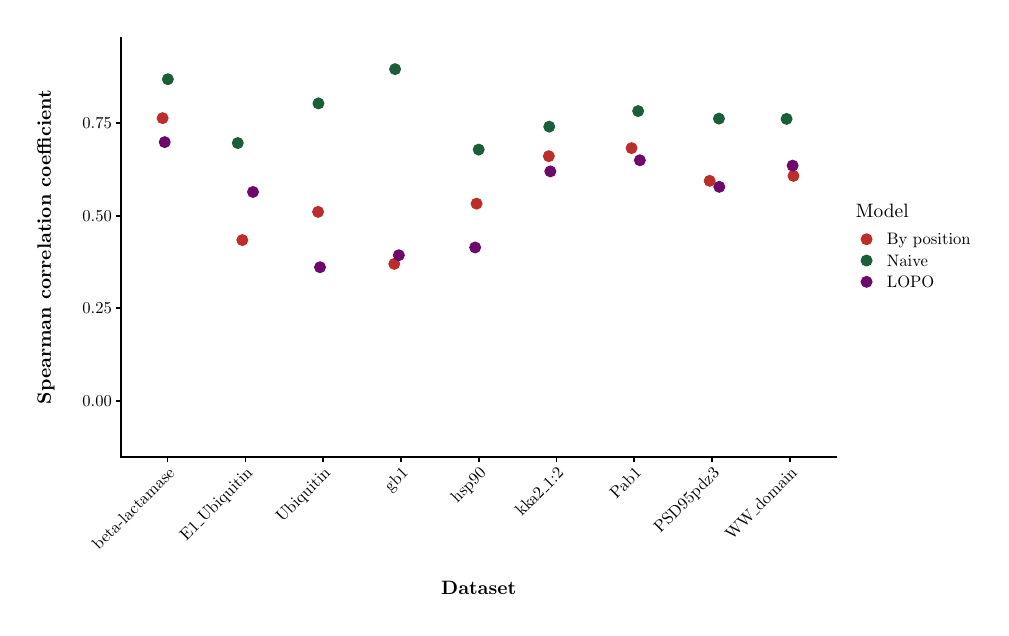
\begin{tikzpicture}[x=1pt,y=1pt]
\definecolor{fillColor}{RGB}{255,255,255}
\path[use as bounding box,fill=fillColor,fill opacity=0.00] (0,0) rectangle (344.26,209.59);
\begin{scope}
\path[clip] ( 33.67, 54.47) rectangle (292.28,206.09);
\definecolor{drawColor}{RGB}{28,94,57}
\definecolor{fillColor}{RGB}{28,94,57}

\path[draw=drawColor,line width= 0.4pt,line join=round,line cap=round,fill=fillColor] ( 75.93,167.90) circle (  1.96);

\path[draw=drawColor,line width= 0.4pt,line join=round,line cap=round,fill=fillColor] (249.80,176.72) circle (  1.96);

\path[draw=drawColor,line width= 0.4pt,line join=round,line cap=round,fill=fillColor] (220.59,179.45) circle (  1.96);

\path[draw=drawColor,line width= 0.4pt,line join=round,line cap=round,fill=fillColor] (105.08,182.22) circle (  1.96);

\path[draw=drawColor,line width= 0.4pt,line join=round,line cap=round,fill=fillColor] (274.23,176.62) circle (  1.96);

\path[draw=drawColor,line width= 0.4pt,line join=round,line cap=round,fill=fillColor] ( 50.66,190.96) circle (  1.96);

\path[draw=drawColor,line width= 0.4pt,line join=round,line cap=round,fill=fillColor] (132.77,194.60) circle (  1.96);

\path[draw=drawColor,line width= 0.4pt,line join=round,line cap=round,fill=fillColor] (162.98,165.53) circle (  1.96);

\path[draw=drawColor,line width= 0.4pt,line join=round,line cap=round,fill=fillColor] (188.47,173.82) circle (  1.96);
\definecolor{drawColor}{RGB}{187,46,41}
\definecolor{fillColor}{RGB}{187,46,41}

\path[draw=drawColor,line width= 0.4pt,line join=round,line cap=round,fill=fillColor] ( 77.57,132.84) circle (  1.96);

\path[draw=drawColor,line width= 0.4pt,line join=round,line cap=round,fill=fillColor] (246.44,154.24) circle (  1.96);

\path[draw=drawColor,line width= 0.4pt,line join=round,line cap=round,fill=fillColor] (218.21,166.07) circle (  1.96);

\path[draw=drawColor,line width= 0.4pt,line join=round,line cap=round,fill=fillColor] (104.93,143.03) circle (  1.96);

\path[draw=drawColor,line width= 0.4pt,line join=round,line cap=round,fill=fillColor] (276.72,156.03) circle (  1.96);

\path[draw=drawColor,line width= 0.4pt,line join=round,line cap=round,fill=fillColor] ( 48.76,176.90) circle (  1.96);

\path[draw=drawColor,line width= 0.4pt,line join=round,line cap=round,fill=fillColor] (132.47,124.24) circle (  1.96);

\path[draw=drawColor,line width= 0.4pt,line join=round,line cap=round,fill=fillColor] (162.21,145.99) circle (  1.96);

\path[draw=drawColor,line width= 0.4pt,line join=round,line cap=round,fill=fillColor] (188.32,163.16) circle (  1.96);
\definecolor{drawColor}{RGB}{108,9,106}
\definecolor{fillColor}{RGB}{108,9,106}

\path[draw=drawColor,line width= 0.4pt,line join=round,line cap=round,fill=fillColor] (188.87,157.66) circle (  1.96);

\path[draw=drawColor,line width= 0.4pt,line join=round,line cap=round,fill=fillColor] (161.69,130.17) circle (  1.96);

\path[draw=drawColor,line width= 0.4pt,line join=round,line cap=round,fill=fillColor] (221.22,161.68) circle (  1.96);

\path[draw=drawColor,line width= 0.4pt,line join=round,line cap=round,fill=fillColor] (134.12,127.36) circle (  1.96);

\path[draw=drawColor,line width= 0.4pt,line join=round,line cap=round,fill=fillColor] (105.64,123.03) circle (  1.96);

\path[draw=drawColor,line width= 0.4pt,line join=round,line cap=round,fill=fillColor] ( 81.42,150.22) circle (  1.96);

\path[draw=drawColor,line width= 0.4pt,line join=round,line cap=round,fill=fillColor] (249.93,152.07) circle (  1.96);

\path[draw=drawColor,line width= 0.4pt,line join=round,line cap=round,fill=fillColor] (276.41,159.74) circle (  1.96);

\path[draw=drawColor,line width= 0.4pt,line join=round,line cap=round,fill=fillColor] ( 49.52,168.23) circle (  1.96);
\end{scope}
\begin{scope}
\path[clip] (  0.00,  0.00) rectangle (344.26,209.59);
\definecolor{drawColor}{RGB}{0,0,0}

\path[draw=drawColor,line width= 0.6pt,line join=round,line cap=rect] ( 33.67, 54.47) --
	( 33.67,206.09);
\end{scope}
\begin{scope}
\path[clip] (  0.00,  0.00) rectangle (344.26,209.59);
\definecolor{drawColor}{RGB}{0,0,0}

\node[text=drawColor,anchor=base east,inner sep=0pt, outer sep=0pt, scale=  0.60] at ( 30.42, 72.68) {0.00};

\node[text=drawColor,anchor=base east,inner sep=0pt, outer sep=0pt, scale=  0.60] at ( 30.42,106.13) {0.25};

\node[text=drawColor,anchor=base east,inner sep=0pt, outer sep=0pt, scale=  0.60] at ( 30.42,139.59) {0.50};

\node[text=drawColor,anchor=base east,inner sep=0pt, outer sep=0pt, scale=  0.60] at ( 30.42,173.04) {0.75};
\end{scope}
\begin{scope}
\path[clip] (  0.00,  0.00) rectangle (344.26,209.59);
\definecolor{drawColor}{RGB}{0,0,0}

\path[draw=drawColor,line width= 0.6pt,line join=round] ( 31.92, 74.74) --
	( 33.67, 74.74);

\path[draw=drawColor,line width= 0.6pt,line join=round] ( 31.92,108.20) --
	( 33.67,108.20);

\path[draw=drawColor,line width= 0.6pt,line join=round] ( 31.92,141.65) --
	( 33.67,141.65);

\path[draw=drawColor,line width= 0.6pt,line join=round] ( 31.92,175.11) --
	( 33.67,175.11);
\end{scope}
\begin{scope}
\path[clip] (  0.00,  0.00) rectangle (344.26,209.59);
\definecolor{drawColor}{RGB}{0,0,0}

\path[draw=drawColor,line width= 0.6pt,line join=round,line cap=rect] ( 33.67, 54.47) --
	(292.28, 54.47);
\end{scope}
\begin{scope}
\path[clip] (  0.00,  0.00) rectangle (344.26,209.59);
\definecolor{drawColor}{RGB}{0,0,0}

\path[draw=drawColor,line width= 0.6pt,line join=round] ( 50.54, 52.72) --
	( 50.54, 54.47);

\path[draw=drawColor,line width= 0.6pt,line join=round] ( 78.65, 52.72) --
	( 78.65, 54.47);

\path[draw=drawColor,line width= 0.6pt,line join=round] (106.76, 52.72) --
	(106.76, 54.47);

\path[draw=drawColor,line width= 0.6pt,line join=round] (134.87, 52.72) --
	(134.87, 54.47);

\path[draw=drawColor,line width= 0.6pt,line join=round] (162.98, 52.72) --
	(162.98, 54.47);

\path[draw=drawColor,line width= 0.6pt,line join=round] (191.09, 52.72) --
	(191.09, 54.47);

\path[draw=drawColor,line width= 0.6pt,line join=round] (219.19, 52.72) --
	(219.19, 54.47);

\path[draw=drawColor,line width= 0.6pt,line join=round] (247.30, 52.72) --
	(247.30, 54.47);

\path[draw=drawColor,line width= 0.6pt,line join=round] (275.41, 52.72) --
	(275.41, 54.47);
\end{scope}
\begin{scope}
\path[clip] (  0.00,  0.00) rectangle (344.26,209.59);
\definecolor{drawColor}{RGB}{0,0,0}

\node[text=drawColor,rotate= 45.00,anchor=base east,inner sep=0pt, outer sep=0pt, scale=  0.60] at ( 53.46, 48.30) {beta-lactamase};

\node[text=drawColor,rotate= 45.00,anchor=base east,inner sep=0pt, outer sep=0pt, scale=  0.60] at ( 81.57, 48.30) {E1\_Ubiquitin};

\node[text=drawColor,rotate= 45.00,anchor=base east,inner sep=0pt, outer sep=0pt, scale=  0.60] at (109.68, 48.30) {Ubiquitin};

\node[text=drawColor,rotate= 45.00,anchor=base east,inner sep=0pt, outer sep=0pt, scale=  0.60] at (137.79, 48.30) {gb1};

\node[text=drawColor,rotate= 45.00,anchor=base east,inner sep=0pt, outer sep=0pt, scale=  0.60] at (165.90, 48.30) {hsp90};

\node[text=drawColor,rotate= 45.00,anchor=base east,inner sep=0pt, outer sep=0pt, scale=  0.60] at (194.01, 48.30) {kka2\_1:2};

\node[text=drawColor,rotate= 45.00,anchor=base east,inner sep=0pt, outer sep=0pt, scale=  0.60] at (222.12, 48.30) {Pab1};

\node[text=drawColor,rotate= 45.00,anchor=base east,inner sep=0pt, outer sep=0pt, scale=  0.60] at (250.23, 48.30) {PSD95pdz3};

\node[text=drawColor,rotate= 45.00,anchor=base east,inner sep=0pt, outer sep=0pt, scale=  0.60] at (278.34, 48.30) {WW\_domain};
\end{scope}
\begin{scope}
\path[clip] (  0.00,  0.00) rectangle (344.26,209.59);
\definecolor{drawColor}{RGB}{0,0,0}

\node[text=drawColor,anchor=base,inner sep=0pt, outer sep=0pt, scale=  0.70] at (162.98,  4.86) {\bfseries Dataset};
\end{scope}
\begin{scope}
\path[clip] (  0.00,  0.00) rectangle (344.26,209.59);
\definecolor{drawColor}{RGB}{0,0,0}

\node[text=drawColor,rotate= 90.00,anchor=base,inner sep=0pt, outer sep=0pt, scale=  0.70] at (  8.39,130.28) {\bfseries Spearman correlation coefficient};
\end{scope}
\begin{scope}
\path[clip] (  0.00,  0.00) rectangle (344.26,209.59);
\definecolor{drawColor}{RGB}{0,0,0}

\node[text=drawColor,anchor=base west,inner sep=0pt, outer sep=0pt, scale=  0.70] at (299.28,141.17) {Model};
\end{scope}
\begin{scope}
\path[clip] (  0.00,  0.00) rectangle (344.26,209.59);
\definecolor{drawColor}{RGB}{187,46,41}
\definecolor{fillColor}{RGB}{187,46,41}

\path[draw=drawColor,line width= 0.4pt,line join=round,line cap=round,fill=fillColor] (303.13,133.14) circle (  1.96);
\end{scope}
\begin{scope}
\path[clip] (  0.00,  0.00) rectangle (344.26,209.59);
\definecolor{drawColor}{RGB}{28,94,57}
\definecolor{fillColor}{RGB}{28,94,57}

\path[draw=drawColor,line width= 0.4pt,line join=round,line cap=round,fill=fillColor] (303.13,125.44) circle (  1.96);
\end{scope}
\begin{scope}
\path[clip] (  0.00,  0.00) rectangle (344.26,209.59);
\definecolor{drawColor}{RGB}{108,9,106}
\definecolor{fillColor}{RGB}{108,9,106}

\path[draw=drawColor,line width= 0.4pt,line join=round,line cap=round,fill=fillColor] (303.13,117.74) circle (  1.96);
\end{scope}
\begin{scope}
\path[clip] (  0.00,  0.00) rectangle (344.26,209.59);
\definecolor{drawColor}{RGB}{0,0,0}

\node[text=drawColor,anchor=base west,inner sep=0pt, outer sep=0pt, scale=  0.60] at (310.48,131.07) {By position};
\end{scope}
\begin{scope}
\path[clip] (  0.00,  0.00) rectangle (344.26,209.59);
\definecolor{drawColor}{RGB}{0,0,0}

\node[text=drawColor,anchor=base west,inner sep=0pt, outer sep=0pt, scale=  0.60] at (310.48,123.37) {Naive};
\end{scope}
\begin{scope}
\path[clip] (  0.00,  0.00) rectangle (344.26,209.59);
\definecolor{drawColor}{RGB}{0,0,0}

\node[text=drawColor,anchor=base west,inner sep=0pt, outer sep=0pt, scale=  0.60] at (310.48,115.67) {LOPO};
\end{scope}
\end{tikzpicture}
